\chapter{Fine-grained Cross Modal Retrieval}
\label{cha:Method}

In Chapter \ref{cha:scan}, we explained in detail on the structure and principle behind our coarse-grained cross modal retrieval model. As we discussed, there are aspects that we can focus on to
%% SHURONG: change the 'improvements here' as stated in several places in previous chapters. 这个model并不novel, 但是我们把针对artworks的fine-grained retrieval 定位为一个novel task[done!]
achieve cross modal retrieval on another level: fine-grained. In this chapter, we present our model for the novel task of fine-grained cross modal retrieval.

The structure of this chapter is as follows. Section 4.1 gives a brief introduction on our plans for modifying the previous model into a fragment level. Section 4.2 explains the processed artwork datasets and why the pre-processing is necessary for our model. Section 4.3 proposes our fine-grained cross modal retrieval model on a fragment level instead of focusing on whole images or sentences. Section 4.4 shows the results of our presented model running on our annotated artworks datasets. Section 4.5 points out some existing shortcomings of our methodology and potential fields to be focused on in the future. Section 4.6 concludes this section.


\section{Fragment Retrieval}
In this chapter, we are trying to solve the cross modal retrieval task at a fine-grained level, which means we shall not limit our retrieval on the image or sentence level but a fragment level. We applied some changes in the previous model in Chapter \ref{cha:scan}:

\begin{itemize}
    \item Instead of attending between image fragments with each token in sentence captions, here we extract noun phrases from sentence captions to perform mutual attention with image fragments in order to find correspondence between the two modalities on fragment level. 
    %% SHURONG:add the purpose of doing this: in order to find fragment-level correspondance between the two modalities.[done]
    \item During the testing process, we replace the original annotations of artworks but adopt manually handcrafted annotations as ground truth, which shall give us a more accurate experiment result.
\end{itemize}

Next, we present our datasets used in this chapter.

\section{Dataset Preparation}
\label{sec:dataprep}
As we mentioned in Chapter \ref{cha:intro}, the same datasets used in this Chapter and Chapter \ref{cha:scan} are from the image caption paper by Sheng et al. \cite{artworkcaption}. For each artwork, two files were available: a high-resolution \verb|jpeg| image file and an accompanying \verb|xml| and \verb|json| file including the metadata.

Python scripts (see Appendix \ref{app:A}) were written to parse the \verb|xml| and \verb|json| files. Instead of using the raw captions, here the textual attributes we use are already processed into phrases. The technique here used is from Handler et al. \cite{nounphrase}, it extracts noun phrases from captions in raw \verb|xml| and \verb|json| files which potentially helped us improve the accuracy as in most cases noun phrases contain more relevant information of artworks.  

As one single artwork can often have more than one annotation existed in its corresponding \verb|xml| file, it is essential to extract all related annotations out and also combine them into one record for training and testing purpose, which saves computational power and simplifies the model input. We generate a combined \verb|.txt| file for each artwork image which contains all related textual attribution then pass it to the noun phrase extraction process in order to achieve the retrieval in a fragment level; results are saved in \verb|json| format. Details are covered in Appendix \ref{app:A}.

Our training tasks are based on these noun phrases and extracted image fragments. The following section demonstrates the architecture of our fine-grained cross modal retrieval model.

\section{Overall Architecture}

The architecture of the fine-grained cross modal retrieval model is depicted in Figure \ref{fig:mainarch}. This model takes full artwork images and full sentence captions as input. The full artwork image input is a (224, 224) sized high-resolution colour picture and the full sentence caption comes from our dataset which contains several descriptions of artworks.

The model has two pipelines processing image and text input from start, for image input, we first detect salient regions as bottom-up attention \cite{bottomup} to extract features from images using faster R-CNN \cite{fasterrcnn} and ResNet-101 \cite{resnet} (mentioned in Section \ref{sec:fasterrcnn}). These obtained image fragments and their representations will be passed into a fully-connected layer, in order to transform them into a joint embedding space with the same dimension of text (i.e. the dimension of GRU explanation in next paragraph).

\begin{figure}[h!]
\centering
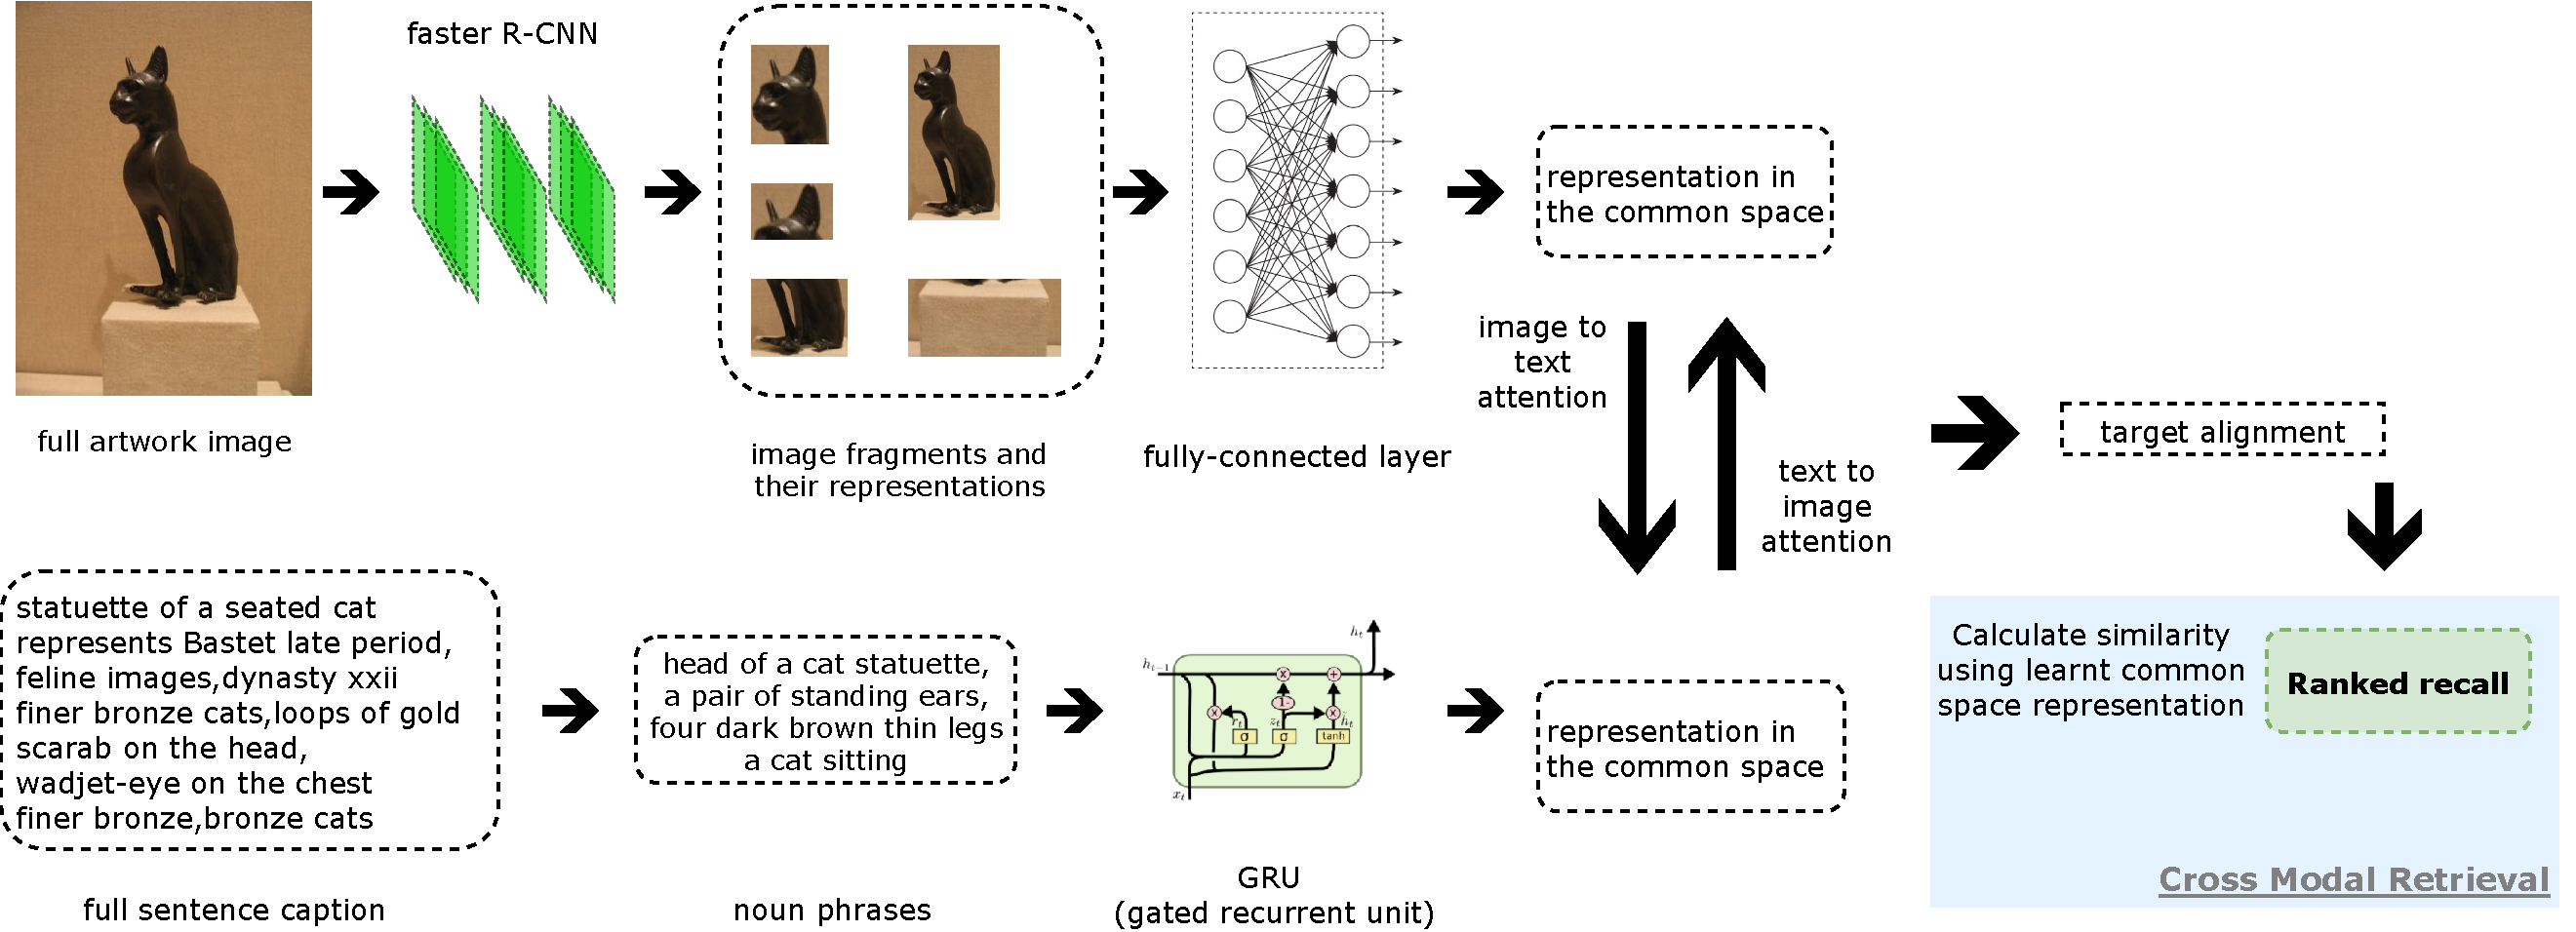
\includegraphics[width=1.0\textwidth]{archinew.pdf}
\caption{Fine-grained Cross Modal Retrieval Model Architecture}
\label{fig:mainarch}
\end{figure}

For full sentence captions as text input, as we mentioned in Section \ref{sec:dataprep}, we do not process the whole sentence directly but first, extract noun phrases out to achieve a finer-grained level. These noun phrases features will be passed into a bidirectional GRU to map them into the same dimension joint embedding space as image features. 

After we learnt image and text representation in a common space, we can use SCAN to attend image to text and attend text to image, in order to get better alignment in between. After computed mutual attention between image and text, we start our follow-up part, which is cross modal retrieval. We use our learnt common space representation to calculate similarity scores between image and text - in this case, cosine similarity; meanwhile, calculate ranked precision and recall for testing.

\section{Experiments}

For experiment settings, we used the same settings and environment as mentioned in Chapter \ref{cha:scan} : Ubuntu machine with Intel Xeon Processor E5-1620 (10M Cache, 3.60 GHz) CPU and a GeForce GTX TITAN X GPU. 

\subsubsection{Settings for image representation}

\begin{itemize}
    \item To save intense labour on retraining model for feature extraction task, we kept the weights pre-trained by Anderson et al. on \verb|Visual Genomes| dataset like in Chapter \ref{cha:scan} for faster R-CNN model and ResNet-101 model and performed detection of salient regions as bottom-up attention to extract features from images. 
    \item We captured $k=36$ Region of Interests (ROIs) for each image after average pooling and extracted 2,048-dimensional features vector.
    \item We used L2 normalisation (Euclidean distance) into 1,024 joint embedding spaces (same for GRU), these will be used as image feature vectors.
\end{itemize}

\subsubsection{Settings for text representation}

\begin{itemize}
    \item We obtained 300-dimensional word embedding as input to GRU then use embedding matrix to map it into 1,024 joint embedding spaces.
\end{itemize}

\subsection{Ground Truth}

For this specific testing task, as we mentioned before, we used our manually annotated ground truth datasets. Each artwork has an updated \verb|xml| file which contains handcrafted image features and textural attributes. Here we show an example of ground truth annotation in Figure \ref{fig:sampledata}.

\begin{figure}[h!]
\centering
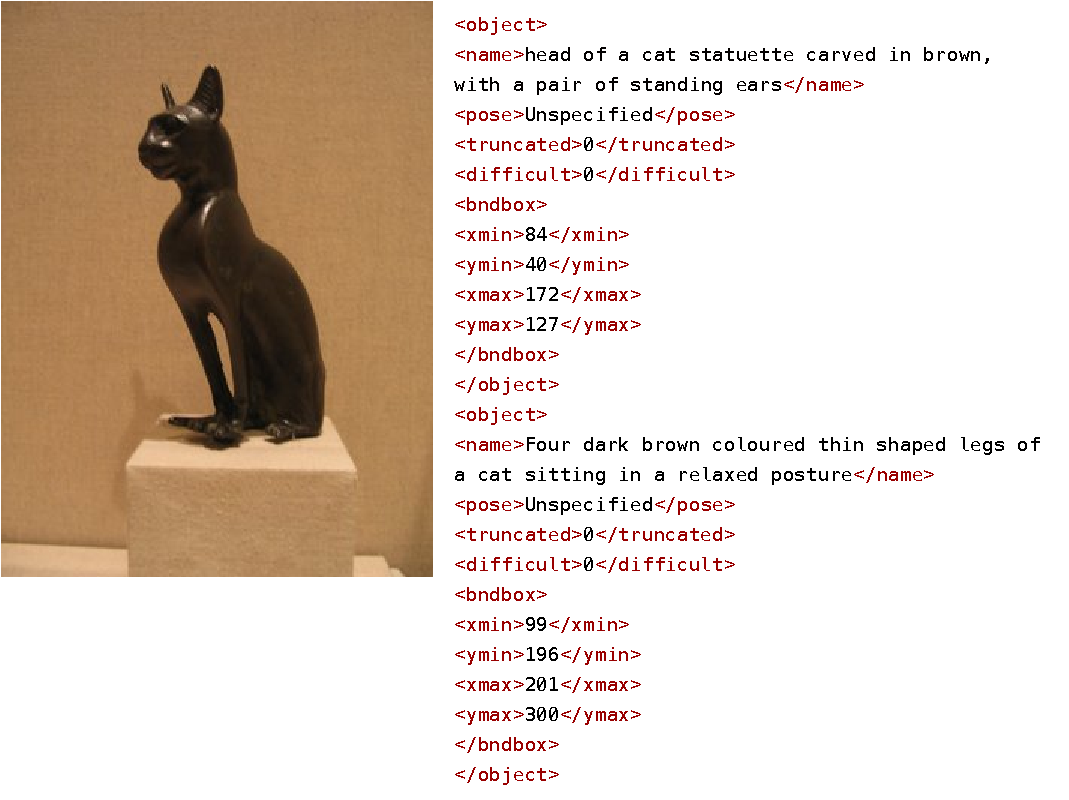
\includegraphics[width=0.8\textwidth]{sampledata.pdf}
\caption{Sample Artwork with Ground Truth Features}
\label{fig:sampledata}
\end{figure}

From Figure \ref{fig:sampledata} we are looking at an Egyptian artwork with a cat sculpture. For all object that exist in the artwork, those are, ``\textit{head of a cat statuette carved in brown, with a pair of standing ears}'' and ``\textit{four dark brown coloured thin shaped legs of a cat sitting in a relaxed posture}'', each of them has a corresponding detailed location, pose, and truncated information attached. 

\subsection{Results}

%%%%%%%%

\begin{table}[h!]
\centering
\begin{tabular}{lcccccc}
\hline
\hline
\multicolumn{1}{c}{} & \multicolumn{3}{c}{Sentence Retrieval} & \multicolumn{3}{c}{Image Retrieval} \\ \hline\hline
\multicolumn{7}{r}{Chinese Artwork Alignment Dataset}                                              \\ \hline
Method               & R@1         & R@5         & R@10       & R@1        & R@5        & R@10      \\ \hline
t-i LSE              & 8.7        & 14.1        & 20.3       & 5.7       & 9.2       & 15.6      \\ \hline
t-i AVG              & 7.9        & 14.4        & 20.6       & 6.2       & 9.6       & 16.2      \\ \hline
i-t LSE              & \textbf{12.8}        & \textbf{20.7}        & 28.7       & \textbf{9.3}       & 15.7       & 22.4      \\ \hline
i-t AVG              & 12.6        & 20.3        & \textbf{28.9}       & 9.1       & \textbf{15.9}       & \textbf{23.2}      \\ \hline
One-directional GRU + i-t AVG  & 15.5        & 18.5        & 24.8       & 7.5       & 14.7       & 19.8      \\ \hline\hline
\multicolumn{7}{r}{Egyptian Artwork Alignment Dataset}                                               \\ \hline
Method               & R@1         & R@5         & R@10       & R@1        & R@5        & R@10      \\ \hline
t-i LSE              & 4.7         & 9.2        & 17.5       & 1.9        & 8.6       & 14.9      \\ \hline
t-i AVG              & 5.1         & 9.4        & 17.9       & 2.2        & 8.9       & 15.2      \\ \hline
i-t LSE              & 5.8         & 11.5        & 20.9       & \textbf{4.7}        & 11.8       & 18.6      \\ \hline
i-t AVG              & \textbf{6.4}         & \textbf{11.6}        & \textbf{21.2}       & 4.4        & \textbf{12.1}       & \textbf{18.7}      \\ \hline
One-directional GRU + i-t AVG  & 5.3         & 10.8        & 20.1       & 3.5        & 10.1       & 16.8      \\ \hline
\end{tabular}
\caption{Result of Fragmented SCAN on Chinese/Egyptian Artwork Dataset}
\label{table:resultfragmented}
\end{table}

Table \ref{table:resultfragmented} present the quantitative results on Chinese and Egyptian artwork datasets where all formulations of our proposed method outperform recent approaches in all measures. Here we denote t-i as Text-Image formulation by text and i-t as Image-Text formulation, AVG as average pooling and LSE as LogSumExp pooling. Like most of the SCAN based models, we tested four different methods by different combinations of formulations and pooling methods. In addition, to check the necessity of bidirectional GRU, we also include a test under one-directional GRU with i-t AVG.

i-t usually surpasses t-i on both pooling methods, and it is evident that using bidirectional GRU improves image annotation R@1 by 2.9 in Chinese artworks and 1.1 in Egyptian artworks, 1.6 and 1.2 for image search. The best result of the model are 13.5 on sentence retrieval (R@1) and 9.9 on image retrieval (R@5) relatively on Chinese artwork dataset; 6.4 on sentence retrieval (R@1) and 4.7 on image retrieval (R@1) relatively on Egyptian artwork dataset. In terms of R@10, our model was able to obtain a 28.6 recall for image annotation task on Chinese dataset which is gratifying and promising considering the strict and detailed ground truth testing set we used.

We noticed that the recalls for sentence and image retrieval on both Chinese and Egyptian artwork datasets are not satisfactorily high. To better understand and evaluate our model, we demonstrate several successful and unsuccessful cross modal retrieval examples in the next section for comparative analysis.

\subsection{Cross Modal Retrieval Examples}
Here we illustrate four typically successful and unsuccessful cross modal retrieval samples of our model: one for each dataset under sentence retrieval and image retrieval. 

\subsubsection{Successful Examples}

\begin{figure}[h!]
\centering
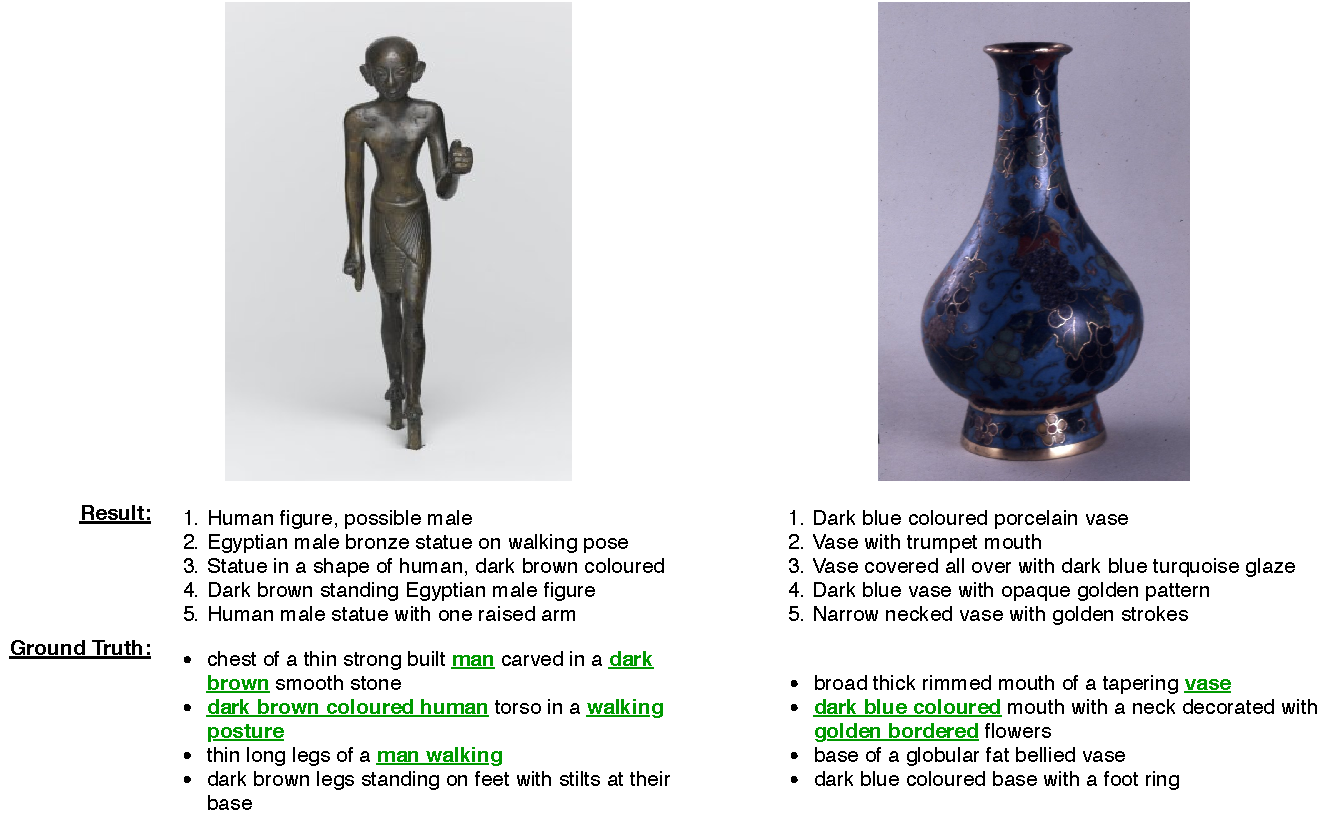
\includegraphics[width=\textwidth]{i2t.pdf}
\caption{Successful Example of Text Phrase Retrieval for Given Image Fragment Queries (fine-grained)}
\label{fig:i2t}
\end{figure}
%%%
Figure \ref{fig:i2t} shows two good text retrieval examples from given image fragment queries. The bottom two Egyptian image fragments achieved excellent retrieval results, the significant features such as colour and shape: ``\textit{grey human face}'', ``\textit{light brown cat head}'' were accurately captured. Although our Egyptian dataset has much more noisy textual information, after obtained noun phrases as input, we noticed that the result was much more detailed; detailed features like ``\textit{big eyes}'', ``\textit{broken nose}'' and ``\textit{standing ears}'' were successfully identified. 

Comparing to those personification figures in Egyptian artworks, our Chinese artwork dataset has more abstract presentations, and some tiny details can be extremely subtle and hard to distinguish from the background. For instance, the top fragment from a traditional Chinese drawing has plentiful features such as those red houses surrounded by trees. Our model was able to pick up almost all of them in a detailed descriptive manner: ``\textit{small houses beside trees}'', ``\textit{black inked inscriptions}''. However, when it comes to sporadically appeared features such as the pattern in the second Chinese artwork fragment, subtle details such as ``\textit{symmetrical flower}'' may be lost although the model still extracted major features like ``\textit{central flower}'' and colours.

\begin{figure}[h!]
\centering
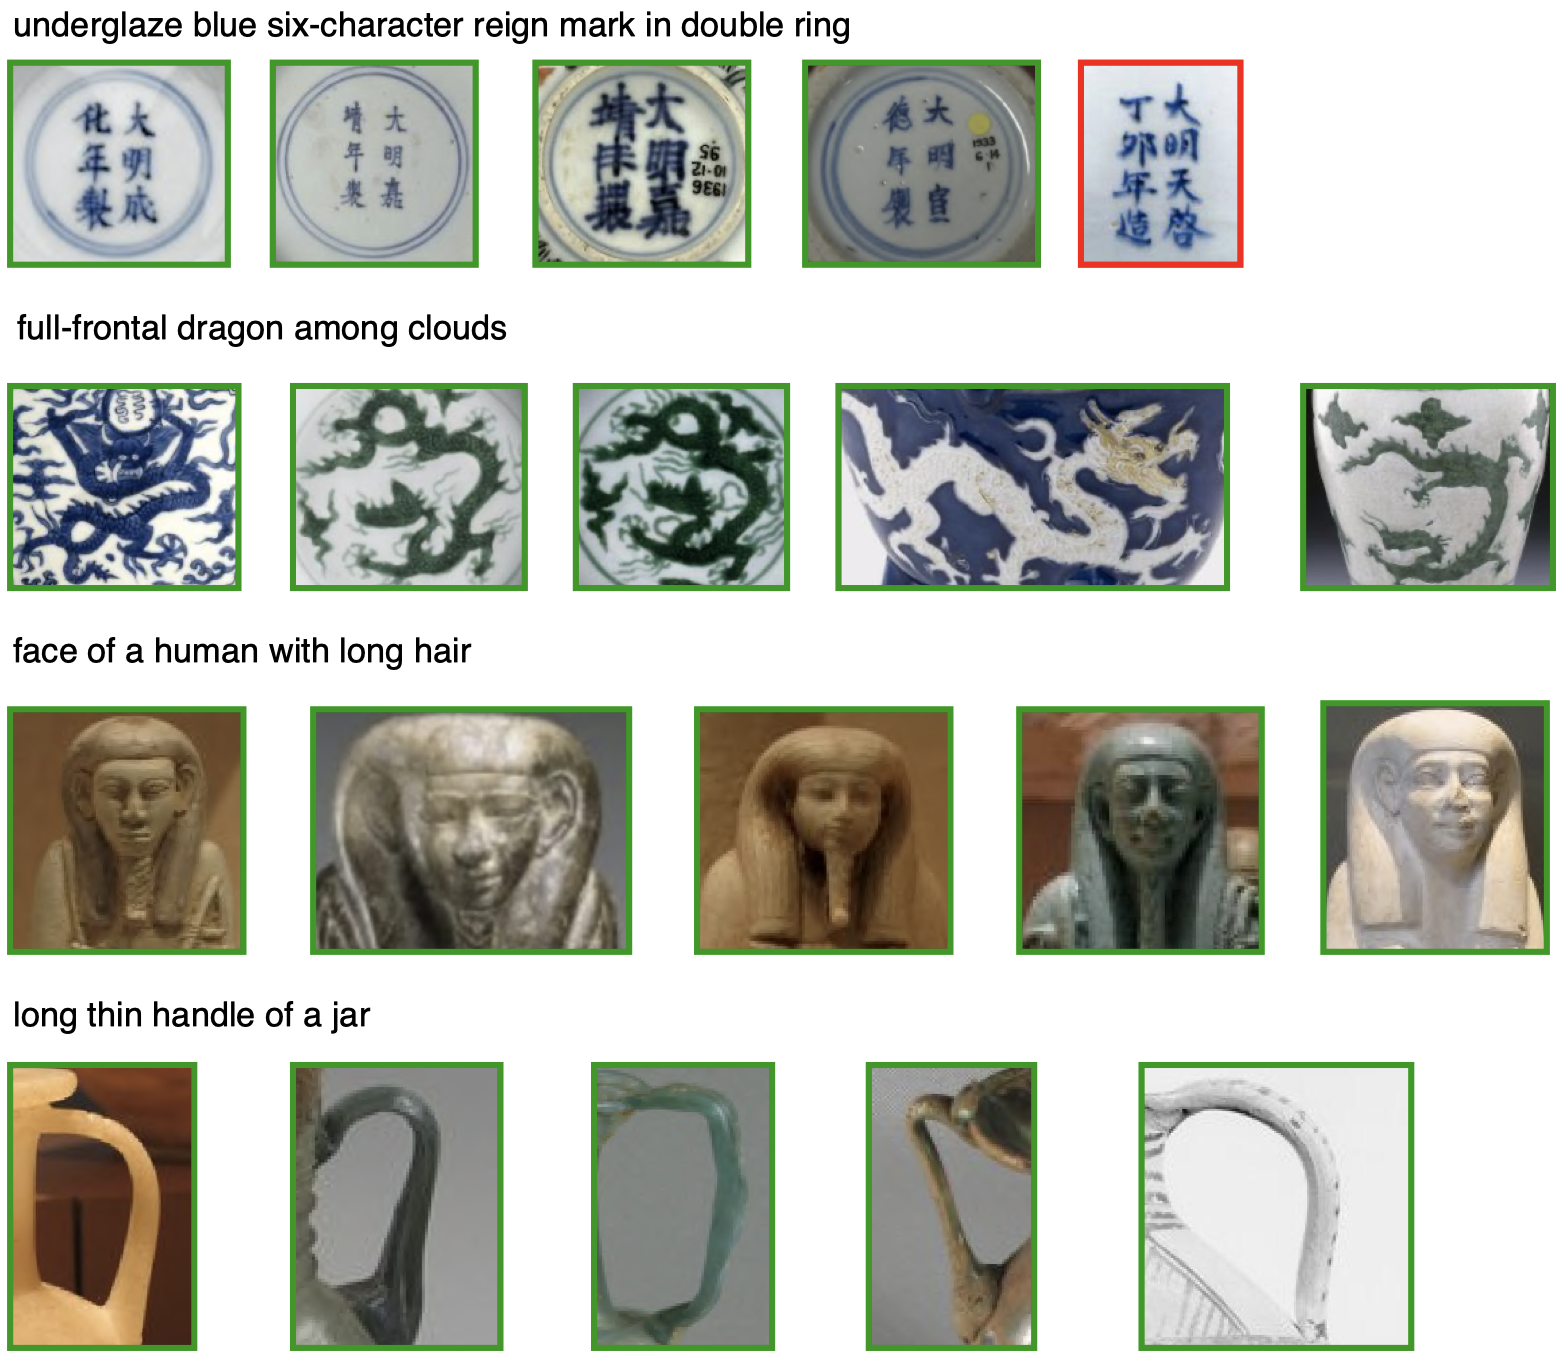
\includegraphics[width=.9\textwidth]{t2i.png}
\caption{Successful Example of Image Fragment Retrieval for Given Text Phrase Queries (fine-grained)}
\label{fig:t2i}
\end{figure}

Next, Figure \ref{fig:t2i} illustrates example image fragment retrieval results from given noun phrase queries. The results from Chinese artwork dataset were impressive as the model successfully distinguished very subtle features from image fragments such as ``\textit{six-character reign mark in double ring}'' and ``\textit{among clouds}''. The bottom two Egyptian noun phrases are fairly simpler than the Chinese ones, significant features such as ``\textit{long hair}'' and ``\textit{long think handle}'' were accurately captured. 

%The top Chinese art text query is very descriptive and detailed, features like ``bridge'' and ``six cross-patterned circles'' helped our model to distinguish the right image from other similar ones. The bottom Egyptian art text queries are fairly easier than the Chinese one as most of the similar artworks differ in shapes and major gestures such as obvious feature ``broken arms raised to the sky''. However, considering the existing irrelevant noun phrases in the Egyptian artwork dataset such as information on Kingdoms and Pharaoh, it is easier for the model to achieve better results on Chinese artwork dataset than the Egyptian one.
\subsubsection{Unsuccessful Examples}

\begin{figure}[h!]
\centering
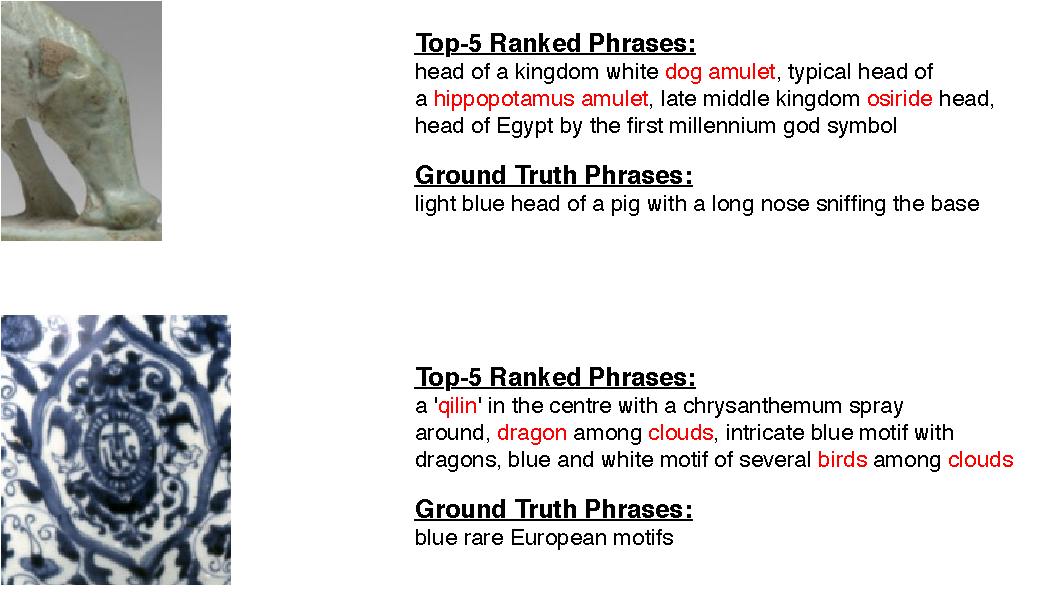
\includegraphics[width=.8\textwidth]{badi2t.pdf}
\caption{Unsuccessful Example of Text Phrase Retrieval for Given Image Fragment Queries (fine-grained)}
\label{fig:badi2t}
\end{figure}

Despite those brilliant fine-grained cross modal retrieval cases we have shown above, here Figure \ref{fig:badi2t} displays two unsuccessful examples noun phrase retrieval results from image fragment queries. Our model was not able to identify the top Egyptian pig amulet head. It has a tricky shape; its rare and unique light-blue colour also made it more difficult for the model to retrieve the correct textual descriptions; our model identified it as a hippopotamus amulet instead. The similar situation happened in the bottom Chinese artwork fragment; European motifs rarely appear in Chinese artworks which misled our model to recognise it as a more widely known figure ``\textit{qilin}''. Our training dataset does not have enough data on this intricate pattern, which raised the difficulty of retrieval task. 

\begin{figure}[h!]
\centering
\includegraphics[width=\textwidth]{badt2i.png}
\caption{Unsuccessful of Image Fragment Retrieval for Given Text Phrase Queries (fine-grained)}
\label{fig:badt2i}
\end{figure}

Finally, Figure \ref{fig:badt2i} demonstrates another four unsuccessful example of image fragment retrieval results from noun phrase queries. Similar to the noun phrase retrieval case we reviewed above, the two samples here also have considerably sporadic features. The model usually can pick up the features such as shape and colour, also repeatedly appeared local characteristics, however, for occasional and distinct local features such as ``\textit{a sword in hand}'', ``\textit{animal shaped bead}'' and ``\textit{pencil sketched mountain}'', the model may get baffled, which lead to inaccurate and inadequate results. For example, the third query requires the painting to be pencil sketched which challenged our model besides the fact that it successfully captured ``\textit{motif of mountain}'' but lost on the ``\textit{pencil sketched}''. Rare features are proved to be more challenging for our model to retrieve.

\subsection{Discussion}
%%
Generally speaking, Chinese artworks surpassed Egyptian artworks on cross modal retrieval tasks - more detailed descriptive noun phrases provided in Chinese artworks. There are still a large amount of irrelevant noisy textual attributes in Egyptian artwork dataset even after noun phrase extraction, which significantly impedes the process of distinguishing features. Subsequently, adequate but not excellent recalls are expected. There are three possible causes:

\begin{itemize}
    \item Our training dataset cannot guarantee a balance of features. For example, there are only 6,000 training images for Chinese artworks, and many of them contain diverse shapes and details. Insufficient training features may influence the ability of the model; therefore, cause inaccurate retrieval results.
    \item As we adopted new ground truth annotations acting testing purpose, considering these features are mostly handcrafted and being almost 100\% accurate, potentially increased the chance of wrong retrieval results which were retrieved based on original raw training phrases obtained from the museum. If we were able to also manually annotate artworks in the training dataset to retrain the model, we suppose the retrieval result shall improve.
    \item One of the crucial requirements for image-text alignment is accurate and proper feature extraction. However, in our case, we used the bottom-up attention mechanism \cite{bottomup}, which was designed and trained on real-world images (\verb|VisualGenome|). We all know that artworks usually have widely different representations and requires unique and specific treatment on feature extraction.
\end{itemize}

Nevertheless, we did not have extra time to redesign our feature learning algorithm to make it more adaptable to artwork representations. To improve our model for better fine-grained cross modal retrieval results, in the next section, we dig into some recent research on the aspect of image-text alignment. 

\section{Future Directions}
In this section, we point out some cutting-edge researches on the field of image-text alignment that are related to our methodology as future directions for further improvements. We are going to discuss in two main directions: the way to align image and text and the way to extract image features (representations).

\subsection{Similarity or Fusion?}
Here we investigated recent research in the field of VQA, the problems of VQA and image-text matching have a lot in common. For example, both accept image and text features as input and then encode. If image-text alignment task is treated as a binary classification problem, the only difference is that the output of VQA task is of multiple classes.

Generally speaking, the processing of image-text matching problems can be divided into ``similarity'' and ``classification''. ``Similarity'' is to use the traditional methods such as cosine similarity or dot product to calculate the similarity between image and text in the same embedding space to judge whether it matches or not. The representative methods are SCAN \cite{scan} and VSRN \cite{VSRN}. The ``classification'' method is to use the neural network to fit a function that is better than the cosine similarity, to determine whether the input image and text feature are a match or not. This input comes from two modes and the output The neural network design for a particular result is generally called ``fusion'', which is more common in VQA, and the representative method is MTFN \cite{MTFN}.

Now let us discuss the pros and cons of traditional similarity calculation and fusion by starting from analysing this problem from a theoretical perspective.

First, we look at a general bilinear fusion method proposed in MUTAN \cite{benyounes2017mutan}:

$$
\text {score}=\sigma\left(\left(x_{\text {img}} \odot x_{\text {txt}}\right) \mathbf{W}\right), x \in \mathcal{R}^{1 \times d}, \mathbf{W} \in \mathcal{R}^{d \times 1}
$$

\begin{figure}[h!]
\centering
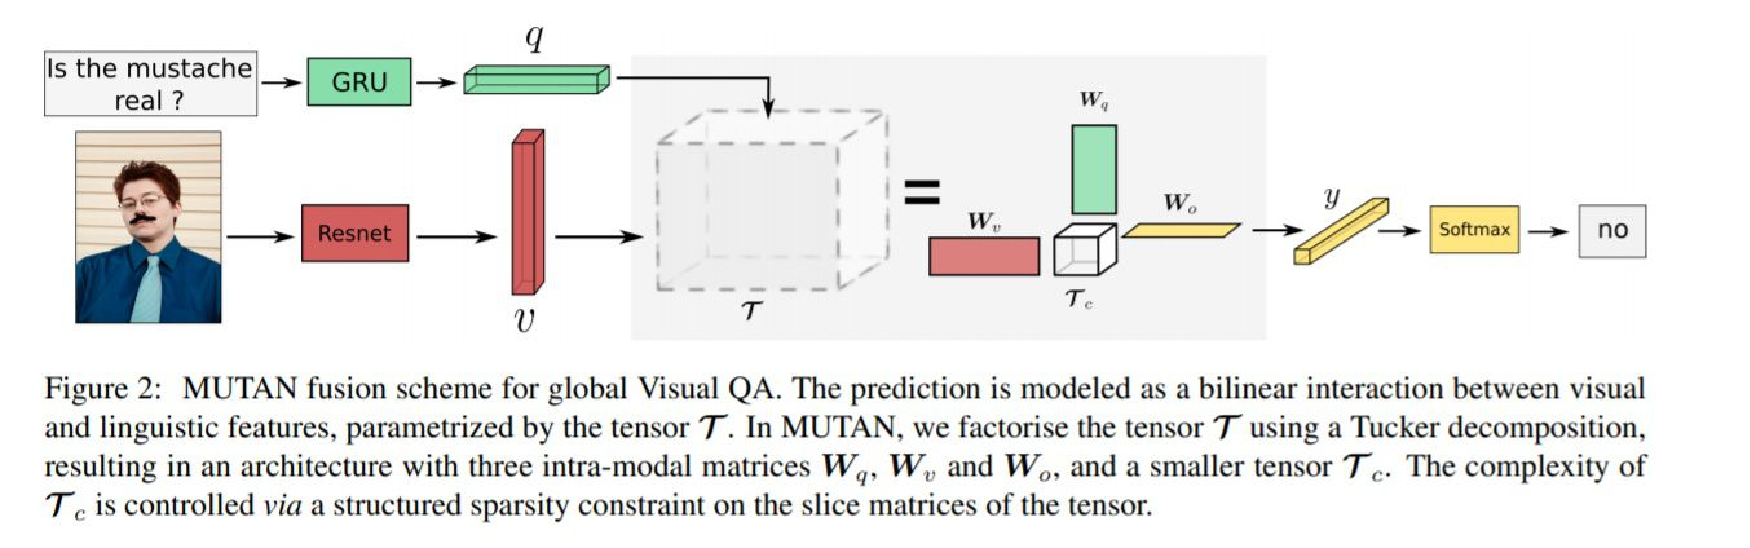
\includegraphics[width=\textwidth]{MUTAN.pdf}
\caption{Bilinear Fusion in MUTAN \cite{benyounes2017mutan}}
\label{fig:mutan}
\end{figure}

Where $x$ represents extracted feature and $\mathbf{W}$ is a learn-able matrix. It is merely to reduce the dimensions after taking the product of the two features and then output the matching probability through the \verb|sigmoid| function. This is also the primary method used in MTFN \cite{MTFN}, which is referred to as bilinear fusion in the following.

Here we use the simplest and most traditional similarity calculation method: dot product here to compare with bilinear fusion:

$$
\text {score}=\sigma\left(x_{\text {img}} x_{t x t}^{\mathrm{T}}\right)
$$

Observing the above two formulas, we can find that bilinear fusion is not much different from the dot product. The dot product is to multiply the corresponding position elements of the two vectors and sum all the elements, while the bilinear fusion is first getting dot product of the corresponding position elements, then get the product of $\mathbf{W}$. This is equivalent to the weighted sum of the elements, that is, when $\mathbf{W}$ is an all-one matrix, bilinear fusion degenerates into a dot product.

From this point of view, bilinear fusion can be understood as weighting different positions when doing dot product when $\mathbf{W}$ is a weight matrix. Weighting helps, but there are two problems:

\begin{itemize}
    \item Optimisation. Can we guarantee a $\mathbf{W}$ better than the all-one matrix?
    \item Design issues. The dimension of the weight matrix is $d\times1$, that is, in the inference, for the element product of any pair of graphic features, the weight of each element position is identical, which is unreasonable.
\end{itemize}

In many experiments, it has not been shown that fusion must perform better than dot product, and dot product is obviously more straightforward and faster than fusion.

\subsubsection{Early Fusion}
There are many improvements to fusion this year, one of the most widely discussed is early fusion. ``Early'' means that comparing to the bilinear fusion mentioned above, it put the multi-modal features into the neural network earlier while there is only one linear layer in bilinear fusion which locates at the end of the entire model. B2T2 \cite{B2T2} compared early fusion and late fusion on the Visual Commonsense Reasoning (VCR) dataset \cite{zellers2019vcr}, and concluded that early fusion usually works better. However, it can be seen from Figure \ref{fig:fusionb2t2} shown below that this comparison can be somewhat unfair, but at least early fusion added more detection information.

\begin{figure}[h!]
\centering
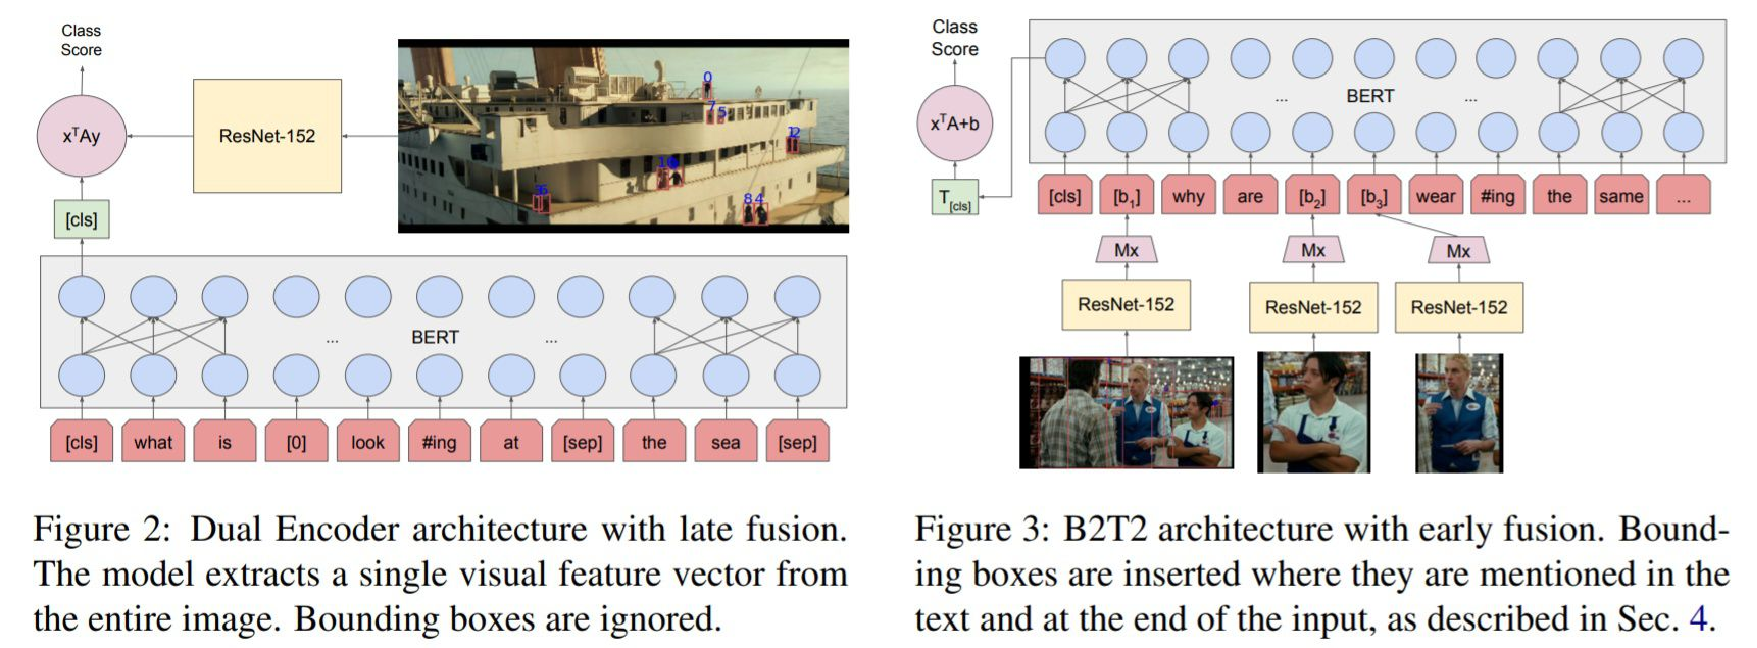
\includegraphics[width=\textwidth]{fusion.pdf}
\caption{Late Fusion (left) \& Early Fusion (right) in B2T2 \cite{B2T2}}
\label{fig:fusionb2t2}
\end{figure}

It should be noted that early fusion is mentioned in many papers, but the structural designs were slightly different, such as RAMEN \cite{ramen}.

Obviously, early fusion has contributed a lot to this aspect, and its performance on VQA is also relatively comparable, but we have not seen enough reliable evidence that early fusion completely exceeds late fusion represented by bilinear fusion. However, at least some aspects have shaken the dominance of bilinear, and these early fusion methods are slightly coarse and have the potential to be better designed. We can expect some future works to break this paradigm.

Back to image-text matching, if the idea of RAMEN \cite{ramen} early fusion is introduced into the research, considerable progress may be made.

\subsection{Better Representation Learning?}

It seems that the most critical factor affecting the alignment task is the characteristics/feature learnt by the network, and the calculation of similarity is not as crucial to a certain extent. VSRN \cite{VSRN} also proved this point by introducing many components to learn features, and then used the most straightforward dot product to achieve the current State-Of-The-Art performance.

Representation learning embodies its importance in earlier work. The bottom-up and top-down \cite{bottomup} attention mechanism used by our previous model has indirectly accomplished many image-text alignment pieces of research. Afterwards, VQA, image-text matching, and image caption all started to use \cite{bottomup} to extract features, which improved SCAN \cite{scan} by a significant amount and shows that a better representation learning model is crucial.

2019 has been a year of the rapid development of representation learning. The leader-board of VCR \cite{zellers2019vcr} has many popular large-scale pre-trained models such as ViBERT \cite{lu2019vilbert}, VideoBERT \cite{sun2019videobert}, UNITE \cite{chen2019uniter} and MoCo \cite{he2019momentum}. Considering the special category of image data we focus on - artworks, here we put more attention on those specialised in artwork feature extraction. Recently, some works \cite{TranslatingArtworks,parttowhole,Art2Real,tan2017artgan,shen2019discovering} have proposed new methodologies for artwork feature extraction and contributed a lot in the field. 


\begin{figure}[h!]
\centering
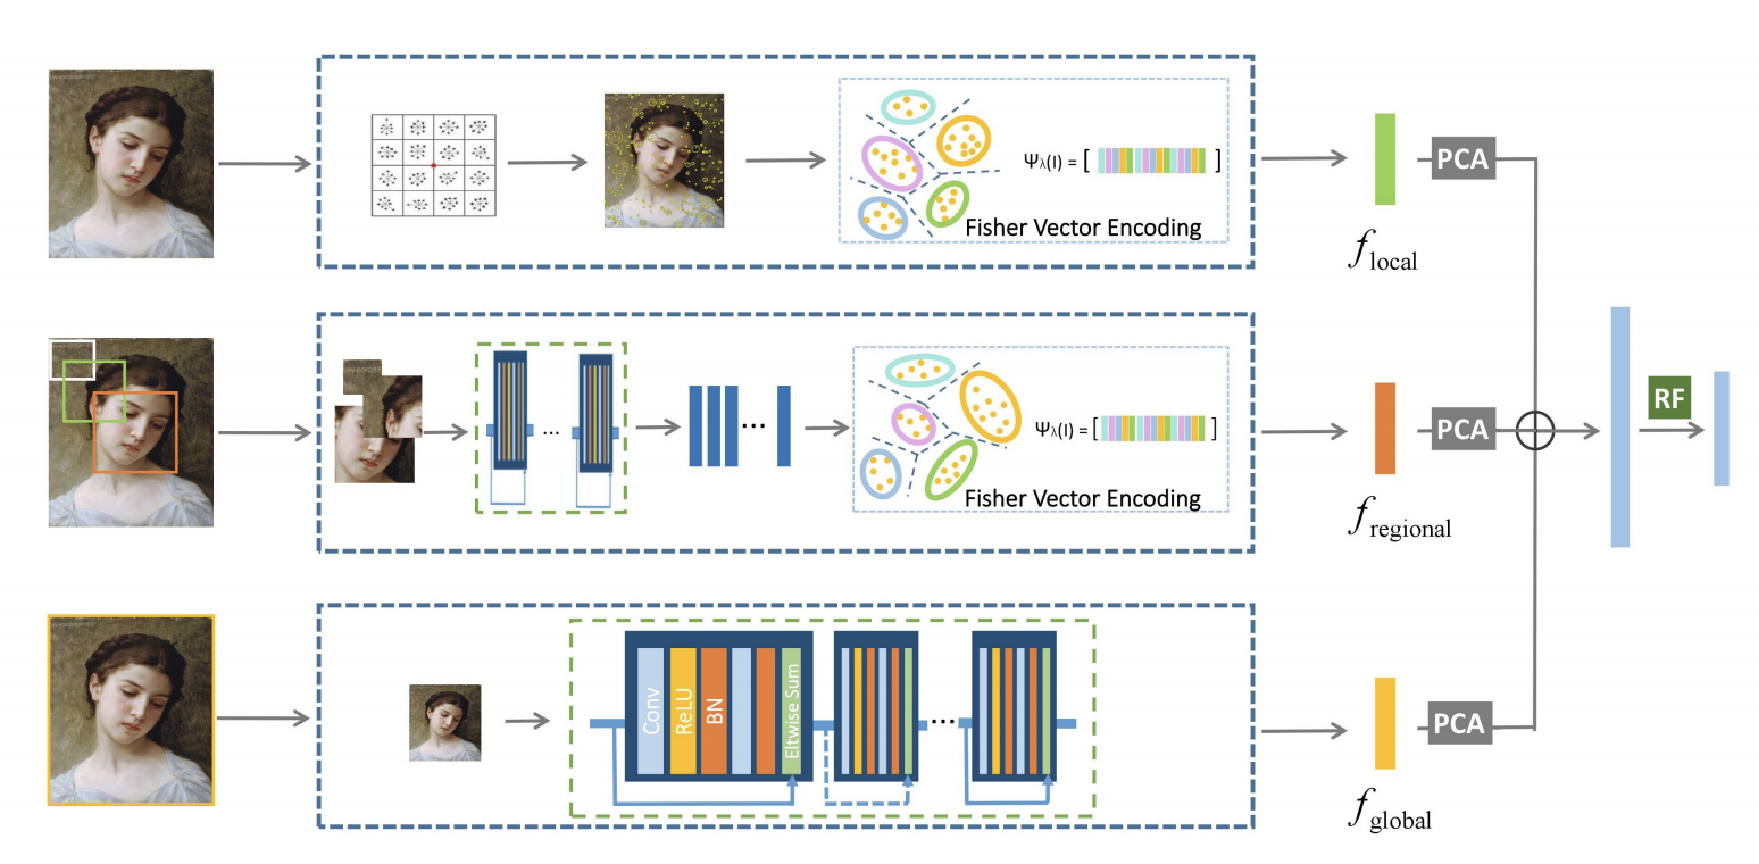
\includegraphics[width=\textwidth]{MTMRoverview.pdf}
\caption{Overview of MTMR Representation Framework \cite{parttowhole}}
\label{fig:mtmroverview}
\end{figure}


Ma el al. \cite{parttowhole} introduced a new methodology for artwork representation in 2017: MTMR (multitask and multi-range). MTMR extracts from the fisher vector based on scale-invariant feature transformation (SIFT) from the painting:

\begin{itemize}
    \item Local, regional and global features
    \item Multiclass area coding structure
    \item Multitask learning framework
\end{itemize}

Figure \ref{fig:mtmroverview} illustrates the overall architecture of the MTMR representation framework. The above, middle and bottom represent different levels of feature extraction using SIFT-based fisher vector: local, regional and global, respectively. Inside each level, there are multiclass area coding and multitask learning structures. These obtained features in different levels will be finally passed to the random forest model as an ensemble mechanism to retrieve a final result.

Figure \ref{fig:mtmrmulti} shows the detailed structure of how multitask learning works in the MTMR framework. The right grey box contains several different tasks which are split to process in parallel. There is a residual network inside the green box, which consists of fully connected layers and convolutional layers for artwork image feature extraction.


\begin{figure}[h!]
\centering
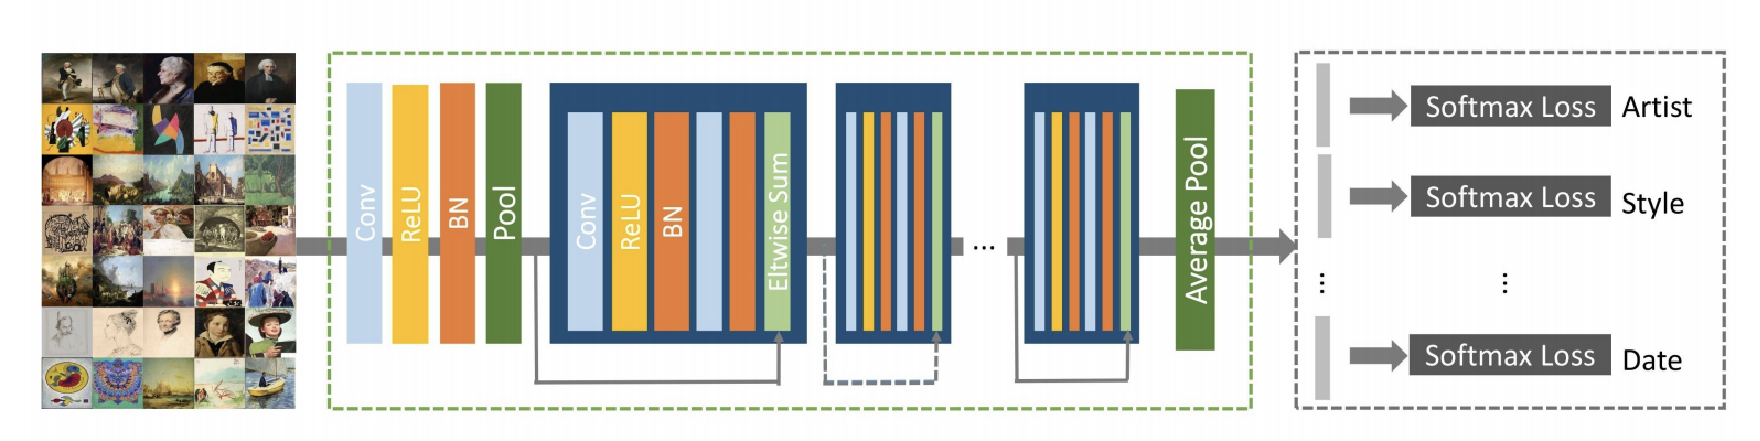
\includegraphics[width=\textwidth]{MTMRmultitask.pdf}
\caption{MTMR's Multitask Learning Structure \cite{parttowhole}}
\label{fig:mtmrmulti}
\end{figure}

Besides the MTMR framework, in 2019, Shen et al. \cite{shen2019discovering} tried to find almost repetitive patterns from a large number of artworks. 

Due to the differences in artistic media (oil paintings, pastel paintings, sketches, etc.) and the inherent deviations in the reproduction process, this goal is more difficult to mine than standard examples. The critical technology is to use self-supervised learning to fine-tune standard depth features on specific art collections to adapt them to this task. Correctly, use spatial consistency between adjacent feature matches as a supervised fine-tuning signal. The adjusted features enable more accurate matching (not affected by differences in style) and can be used with standard pattern discovery methods based on geometric verification to identify repeating patterns in the dataset.

\begin{figure}[h!]
\centering
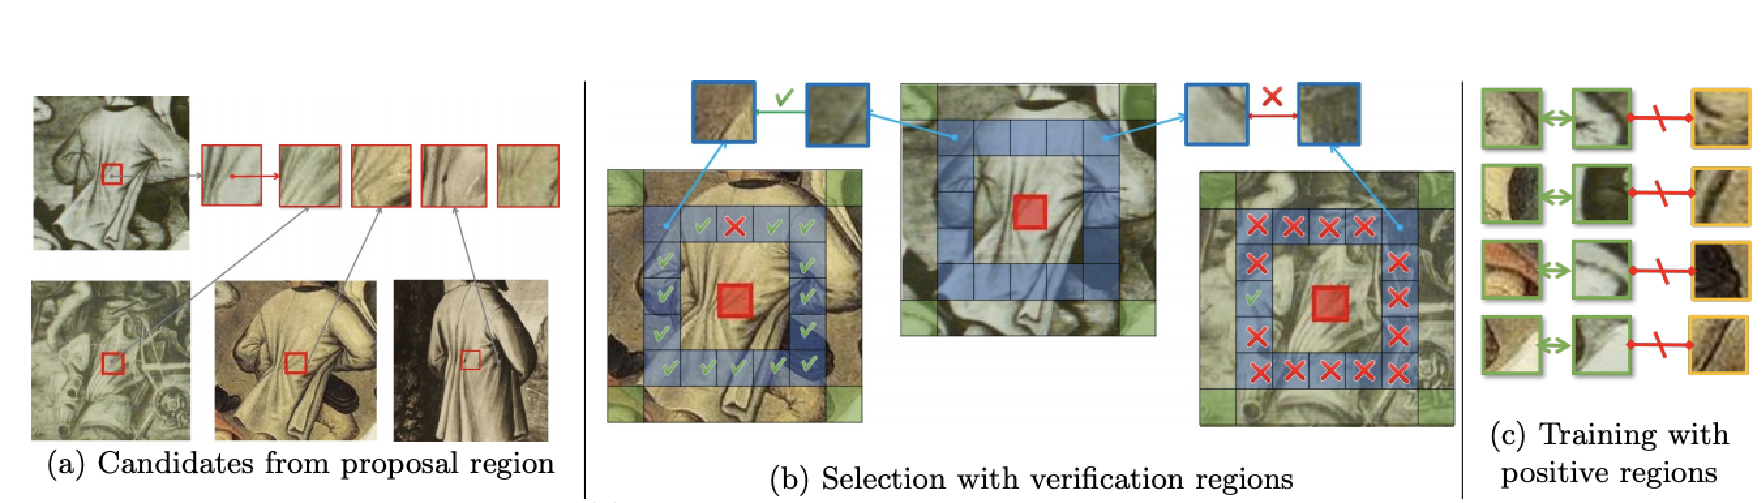
\includegraphics[width=\textwidth]{featurelearningartwork.pdf}
\caption{Feature Learning Strategy \cite{shen2019discovering}}
\label{fig:featurelearning}
\end{figure}

Figure \ref{fig:featurelearning} demonstrates the feature learning process proposed. First candidate correspondences need to be obtained, which come from matching the proposal regions in red boxes with the original complete dataset. Next, these correspondences are checked by comparing features from validation regions (in blue). Finally, only positive results from the previous step will be extracted and kept. 

The method is evaluated on multiple different datasets and showed significant qualitative findings. In terms of quantitative evaluation, the researchers marked 273 approximately repeating details in the dataset of 1,587 works of art by Lao Jan Bruegel and his studio. In addition to works of art, the researchers also showed improvements in the positioning of the algorithm on the \verb|Oxford5K| photo dataset \cite{Philbin07} and historical photo positioning on the LTLL (Large Time Lags Location) dataset \cite{Fernando2015CVIU}.

We believe that a multitasking framework focusing on different levels of features like MTMR \cite{parttowhole} along with a fine-grained feature matching strategies mentioned in Shen et al.'s research \cite{shen2019discovering} will significantly help improve the fine-grained cross modal retrieval model.

\section{Conclusion}
In this chapter, we first presented a fine-grained cross modal retrieval model based on SCAN. It enables image-text retrieval on a fragment level which potentially eased the artwork annotation task. Next, we conducted several experiments under different settings to test the performance of our model on Egyptian and Chinese datasets by comparing their recall rates. To better illustrate and explain the results, we displayed several successful and unsuccessful retrieval examples from our experiments, which shows our model has the ability to pick commonly shared features out accurately but sometimes gets stuck on rare and unique features. Lack of enough artwork training examples is also suspected as a cause of adequate recalls. We finally pointed out future directions on the image-text alignment task by investigating recent research works and proposed two significant aspects that could benefit our model.

%%% Local Variables: 
%%% mode: latex
%%% TeX-master: "thesis"
%%% End: 
